\documentclass{beamer}
\usepackage[utf8]{inputenc}

\usetheme{Madrid}
\usecolortheme{default}
\usepackage{amsmath,amssymb,amsfonts,amsthm}
\usepackage{txfonts}
\usepackage{tkz-euclide}
\usepackage{listings}
\usepackage{adjustbox}
\usepackage{array}
\usepackage{tabularx}
\usepackage{gvv}
\usepackage{lmodern}
\usepackage{circuitikz}
\usepackage{tikz}
\usepackage{graphicx}

\setbeamertemplate{page number in head/foot}[totalframenumber]

\usepackage{tcolorbox}
\tcbuselibrary{minted,breakable,xparse,skins}



\definecolor{bg}{gray}{0.95}
\DeclareTCBListing{mintedbox}{O{}m!O{}}{%
  breakable=true,
  listing engine=minted,
  listing only,
  minted language=#2,
  minted style=default,
  minted options={%
    linenos,
    gobble=0,
    breaklines=true,
    breakafter=,,
    fontsize=\small,
    numbersep=8pt,
    #1},
  boxsep=0pt,
  left skip=0pt,
  right skip=0pt,
  left=25pt,
  right=0pt,
  top=3pt,
  bottom=3pt,
  arc=5pt,
  leftrule=0pt,
  rightrule=0pt,
  bottomrule=2pt,
  toprule=2pt,
  colback=bg,
  colframe=orange!70,
  enhanced,
  overlay={%
    \begin{tcbclipinterior}
    \fill[orange!20!white] (frame.south west) rectangle ([xshift=20pt]frame.north west);
    \end{tcbclipinterior}},
  #3,
}
\lstset{
    language=C,
    basicstyle=\ttfamily\small,
    keywordstyle=\color{blue},
    stringstyle=\color{orange},
    commentstyle=\color{green!60!black},
    numbers=left,
    numberstyle=\tiny\color{gray},
    breaklines=true,
    showstringspaces=false,
}
%------------------------------------------------------------
%This block of code defines the information to appear in the
%Title page
\title %optional
{4.7.46}
\date{}
%\subtitle{A short story}

\author % (optional)
{Sai Krishna Bakki - EE25BTECH11049}

\begin{document}
\frame{\titlepage}
\begin{frame}{Question}
The equations of the lines passing through the point (1, 0) and at a distance $\frac{\sqrt{3}}{2}$ from the origin, are
\end{frame}
\begin{frame}{Theoretical Solution}
   Given:
\begin{align}
    \vec{A}=\myvec{1\\0},p=\frac{\sqrt{3}}{2}
\end{align}
where p is the perpendicular distance from origin to line and $\vec{A}$ lies on the line.\\
$\therefore$The equation of line in normal form:
\begin{align}
    \myvec{\cos\theta & \sin\theta}\vec{x}=p
\end{align}
substituting $\vec{A}$ and p in line equation gives you:
\begin{align}
    \myvec{\cos\theta & \sin\theta}\myvec{1\\0}=\frac{\sqrt{3}}{2}\\
\end{align}
\end{frame}
\begin{frame}{Theoretical Solution}
we get
\begin{align}
    \cos\theta=\frac{\sqrt{3}}{2}\implies \theta=\frac{\pi}{6}\quad or \quad \frac{-\pi}{6}
\end{align}
Substituting $\theta=\frac{\pi}{6}\quad and \quad \frac{-\pi}{6}$ in $\brak{0.2}$,we get\\
The equations of lines are:
\begin{align}
    \myvec{\frac{\sqrt{3}}{2} & \frac{1}{2}}\vec{x}=\frac{\sqrt{3}}{2}\\
    \myvec{\frac{\sqrt{3}}{2} & -\frac{1}{2}}\vec{x}=\frac{\sqrt{3}}{2}
\end{align}
OR
\begin{align}
 \myvec{\sqrt{3} & 1}\vec{x}=\sqrt{3},
    \myvec{\sqrt{3} & -1}\vec{x}=\sqrt{3}   
\end{align}
\end{frame}
\begin{frame}[fragile]
\frametitle{C Code}
\begin{lstlisting}
#include<stdio.h>
#include<math.h>
int calculate_line_normals(double px, double py, double d,
                           double* out_a1, double* out_b1,
                           double* out_a2, double* out_b2) {

    // 1. Construct the symmetric matrix M = P*P^T - d^2*I
    double M11 = px*px - d*d;
    double M12 = px*py;
    double M22 = py*py - d*d;

    // 2. Find the eigenvalues of M by solving the characteristic equation:
    //    lambda^2 - trace(M)*lambda + det(M) = 0
    double trace = M11 + M22;
    double det = M11 * M22 - M12 * M12;

    double discriminant_lambda = trace*trace - 4*det;
\end{lstlisting}    
\end{frame}
\begin{frame}[fragile]
\frametitle{C Code }
\begin{lstlisting}

    if (discriminant_lambda < 0) {
        // This should not happen for a real symmetric matrix
        return -1;
    }
    double sqrt_discriminant_lambda = sqrt(discriminant_lambda);
    double lambda1 = (trace + sqrt_discriminant_lambda) / 2.0; // Larger eigenvalue
    double lambda2 = (trace - sqrt_discriminant_lambda) / 2.0; // Smaller eigenvalue

    // 3. Check for real solutions. If det > 0, eigenvalues have the same sign.
    //    This means -lambda2/lambda1 is negative, leading to no real solution.
    //    This corresponds to the point P being inside the circle of radius d.
    \end{lstlisting}    
\end{frame}
\begin{frame}[fragile]
\frametitle{C Code }
\begin{lstlisting}
    if (det > 0.0) {
        return -1; // No real lines exist
    }

    // 4. Find the (non-normalized) eigenvector v1 for lambda1
    double v1_x = M12;
    double v1_y = lambda1 - M11;
    // Normalize v1
    double norm_v1 = sqrt(v1_x*v1_x + v1_y*v1_y);
    if (norm_v1 < 1e-9) { // Handle case where eigenvector is zero (M is diagonal)
        v1_x = 1.0; v1_y = 0.0; // A valid eigenvector
    } else {
        v1_x /= norm_v1; v1_y /= norm_v1;
    }


    // 5. Find the (non-normalized) eigenvector v2 for lambda2. Since M is
\end{lstlisting}    
\end{frame}
\begin{frame}[fragile]
\frametitle{C Code }
\begin{lstlisting}
    //    symmetric, v2 is orthogonal to v1.
    double v2_x = -v1_y;
    double v2_y = v1_x;

    // 6. The solution vectors (our normals) are a specific linear combination
    //    of the normalized eigenvectors.
    double sqrt_l1 = sqrt(lambda1);
    double sqrt_neg_l2 = sqrt(-lambda2);

    double n1_x = sqrt_neg_l2 * v1_x + sqrt_l1 * v2_x;
    double n1_y = sqrt_neg_l2 * v1_y + sqrt_l1 * v2_y;
    
    double n2_x = sqrt_neg_l2 * v1_x - sqrt_l1 * v2_x;
    double n2_y = sqrt_neg_l2 * v1_y - sqrt_l1 * v2_y;

    // 7. Set the output values.
    *out_a1 = n1_x;
\end{lstlisting}    
\end{frame}
\begin{frame}[fragile]
\frametitle{C Code }
\begin{lstlisting}
    *out_b1 = n1_y;
    *out_a2 = n2_x;
    *out_b2 = n2_y;

    return 0; // Success
}
\end{lstlisting}    
\end{frame}
\begin{frame}[fragile]
\frametitle{Python code through Shared Output }
\begin{lstlisting}
import ctypes
import numpy as np
import matplotlib.pyplot as plt
from libs.funcs import line_dir_pt
from libs.params import omat
import os

# --- 1. Load the C Shared Library ---
try:
    # Construct the full path to the library file
    lib_path = os.path.join(os.path.dirname(os.path.abspath(__file__)), 'line.so')
    line_lib = ctypes.CDLL(lib_path)
except OSError as e:
    print(f"Error loading shared library: {e}")
    print("Please compile the C code first using 'make'.")
    exit()
\end{lstlisting}    
\end{frame}
\begin{frame}[fragile]
\frametitle{Python code through Shared Output }
\begin{lstlisting}
# --- 2. Define the C Function Signature ---
# Specify the argument types and return type for the C function
calculate_line_normals = line_lib.calculate_line_normals
calculate_line_normals.argtypes = [
    ctypes.c_double, ctypes.c_double, ctypes.c_double,
    ctypes.POINTER(ctypes.c_double), ctypes.POINTER(ctypes.c_double),
    ctypes.POINTER(ctypes.c_double), ctypes.POINTER(ctypes.c_double)
]
calculate_line_normals.restype = ctypes.c_int

# --- 3. Prepare Inputs and Outputs for the C Function ---
# Given point and distance
P_coords = (1.0, 0.0)
d = np.sqrt(3) / 2
\end{lstlisting}    
\end{frame}
\begin{frame}[fragile]
\frametitle{Python code through Shared Output }
\begin{lstlisting}
# Create C-compatible double types for the outputs
a1, b1 = ctypes.c_double(), ctypes.c_double()
a2, b2 = ctypes.c_double(), ctypes.c_double()

# --- 4. Call the C Function ---
result = calculate_line_normals(
    P_coords[0], P_coords[1], d,
    ctypes.byref(a1), ctypes.byref(b1),
    ctypes.byref(a2), ctypes.byref(b2)
)

if result != 0:
    print("C function failed to find a solution.")
    exit()

# --- 5. Process the Results ---
# Convert the results from C types to NumPy arrays
n1 = np.array([a1.value, b1.value]).reshape(-1, 1)
n2 = np.array([a2.value, b2.value]).reshape(-1, 1)
\end{lstlisting}    
\end{frame}
\begin{frame}[fragile]
\frametitle{Python code through Shared Output }
\begin{lstlisting}
# The point through which the lines pass
P = np.array([P_coords[0], P_coords[1]]).reshape(-1, 1)

# Calculate direction vectors by rotating the normal vectors
m1 = omat @ n1
m2 = omat @ n2

# Generate points for plotting the lines
line1 = line_dir_pt(m1, P, k1=-2, k2=2)
line2 = line_dir_pt(m2, P, k1=-2, k2=2)

# --- 6. Plotting ---
plt.figure(figsize=(8, 8))
plt.plot(line1[0, :], line1[1, :], label=r'$\sqrt{3}x + y - \sqrt{3} = 0$')
plt.plot(line2[0, :], line2[1, :], label=r'$\sqrt{3}x - y - \sqrt{3} = 0$')
plt.plot(P[0], P[1], 'o', color='red', markersize=8, label=f'Point P{P_coords}')
\end{lstlisting}    
\end{frame}
\begin{frame}[fragile]
\frametitle{Python code through Shared Output }
\begin{lstlisting}
circle = plt.Circle((0, 0), d, color='gray', linestyle='--', fill=False, label=f'Distance d ≈ {d:.2f}')
plt.gca().add_artist(circle)

plt.axhline(0, color='black', linewidth=1)
plt.axvline(0, color='black', linewidth=1)
plt.title(r"Lines through (1, 0) at a distance of $\frac{\sqrt{3}}{2}$ from the Origin (C Backend)")
plt.xlabel("x-axis")
plt.ylabel("y-axis")
plt.grid(True)
plt.legend()
plt.axis('equal')
plt.xlim(-1.5, 2.5)
plt.ylim(-2, 2)
plt.show()
\end{lstlisting}    
\end{frame}
\begin{frame}[fragile]
\frametitle{Python code}
\begin{lstlisting}
import numpy as np
import matplotlib.pyplot as plt
from libs.funcs import line_dir_pt
from libs.params import omat # Import the rotation matrix

# --- Mathematical Setup ---
# The equation of a line is n.T * x = p.
# We are given a point P(1, 0) on the line and distance from origin d = sqrt(3)/2.
# From the derivation, we found the relationship a^2 = 3*b^2 for the normal vector n = [a, b].T.
# We choose a=sqrt(3), which gives b = +/-1.
n1 = np.array([np.sqrt(3), 1]).reshape(-1, 1)
n2 = np.array([np.sqrt(3), -1]).reshape(-1, 1)

# The point through which the lines pass
P = np.array([1, 0]).reshape(-1, 1)
O = np.array([0, 0]).reshape(-1, 1)
d = np.sqrt(3)/2
\end{lstlisting}    
\end{frame}
\begin{frame}[fragile]
\frametitle{Python code}
\begin{lstlisting}
# --- Line Generation ---
# The direction vector 'm' of a line is perpendicular to its normal vector 'n'.
# We find 'm' by rotating 'n' by 90 degrees using the 'omat' matrix.
m1 = omat @ n1
m2 = omat @ n2

# Generate points for the two lines using the direction vector and the point P.
line1 = line_dir_pt(m1, P, k1=-2, k2=2)
line2 = line_dir_pt(m2, P, k1=-2, k2=2)

# --- Plotting ---
plt.figure(figsize=(8, 8))
\end{lstlisting}    
\end{frame}
\begin{frame}[fragile]
\frametitle{Python code}
\begin{lstlisting}
# Plot the two lines
plt.plot(line1[0, :], line1[1, :], label=r'$\sqrt{3}x + y - \sqrt{3} = 0$')
plt.plot(line2[0, :], line2[1, :], label=r'$\sqrt{3}x - y - \sqrt{3} = 0$')

# Plot the point P and the Origin O
plt.plot(P[0], P[1], 'o', color='red', markersize=8, label='Point P(1, 0)')
plt.plot(O[0], O[1], 'o', color='black', markersize=8, label='Origin O(0, 0)')

# To verify the distance, plot a circle with radius d centered at the origin.
# The lines should appear tangent to this circle.
circle = plt.Circle((0, 0), d, color='gray', linestyle='--', fill=False, label=f'Distance d ≈ {d:.2f}')
plt.gca().add_artist(circle)
\end{lstlisting}    
\end{frame}
\begin{frame}[fragile]
\frametitle{Python code}
\begin{lstlisting}
# --- Plot Customization ---
plt.axhline(0, color='black', linewidth=1)
plt.axvline(0, color='black', linewidth=1)
plt.title(r"Lines through (1, 0) at a distance of $\frac{\sqrt{3}}{2}$ from the Origin")
plt.xlabel("x-axis")
plt.ylabel("y-axis")
plt.grid(True)
plt.legend()
plt.axis('equal') # Ensures correct aspect ratio
plt.xlim(-1.5, 2.5)
plt.ylim(-2, 2)
plt.show()
\end{lstlisting}
\end{frame}
\begin{frame}{Plot By C code and Python Code}
    \begin{figure}
    \centering
    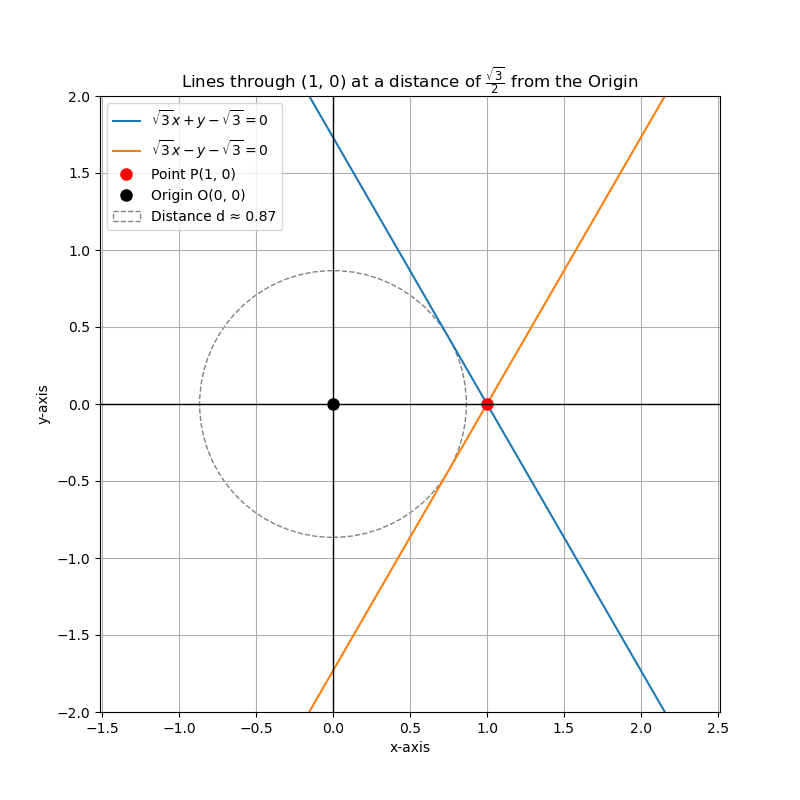
\includegraphics[width=0.7\columnwidth]{figs/Figure_1.png}
    \label{fig:placeholder}
    \caption{1}
\end{figure}
\end{frame}
\end{document}
